% Options for packages loaded elsewhere
\PassOptionsToPackage{unicode}{hyperref}
\PassOptionsToPackage{hyphens}{url}
%
\documentclass[
  ignorenonframetext,
]{beamer}
\usepackage{pgfpages}
\setbeamertemplate{caption}[numbered]
\setbeamertemplate{caption label separator}{: }
\setbeamercolor{caption name}{fg=normal text.fg}
\beamertemplatenavigationsymbolsempty
% Prevent slide breaks in the middle of a paragraph
\widowpenalties 1 10000
\raggedbottom
\setbeamertemplate{part page}{
  \centering
  \begin{beamercolorbox}[sep=16pt,center]{part title}
    \usebeamerfont{part title}\insertpart\par
  \end{beamercolorbox}
}
\setbeamertemplate{section page}{
  \centering
  \begin{beamercolorbox}[sep=12pt,center]{part title}
    \usebeamerfont{section title}\insertsection\par
  \end{beamercolorbox}
}
\setbeamertemplate{subsection page}{
  \centering
  \begin{beamercolorbox}[sep=8pt,center]{part title}
    \usebeamerfont{subsection title}\insertsubsection\par
  \end{beamercolorbox}
}
\AtBeginPart{
  \frame{\partpage}
}
\AtBeginSection{
  \ifbibliography
  \else
    \frame{\sectionpage}
  \fi
}
\AtBeginSubsection{
  \frame{\subsectionpage}
}
\usepackage{amsmath,amssymb}
\usepackage{lmodern}
\usepackage{ifxetex,ifluatex}
\ifnum 0\ifxetex 1\fi\ifluatex 1\fi=0 % if pdftex
  \usepackage[T1]{fontenc}
  \usepackage[utf8]{inputenc}
  \usepackage{textcomp} % provide euro and other symbols
\else % if luatex or xetex
  \usepackage{unicode-math}
  \defaultfontfeatures{Scale=MatchLowercase}
  \defaultfontfeatures[\rmfamily]{Ligatures=TeX,Scale=1}
\fi
% Use upquote if available, for straight quotes in verbatim environments
\IfFileExists{upquote.sty}{\usepackage{upquote}}{}
\IfFileExists{microtype.sty}{% use microtype if available
  \usepackage[]{microtype}
  \UseMicrotypeSet[protrusion]{basicmath} % disable protrusion for tt fonts
}{}
\makeatletter
\@ifundefined{KOMAClassName}{% if non-KOMA class
  \IfFileExists{parskip.sty}{%
    \usepackage{parskip}
  }{% else
    \setlength{\parindent}{0pt}
    \setlength{\parskip}{6pt plus 2pt minus 1pt}}
}{% if KOMA class
  \KOMAoptions{parskip=half}}
\makeatother
\usepackage{xcolor}
\IfFileExists{xurl.sty}{\usepackage{xurl}}{} % add URL line breaks if available
\IfFileExists{bookmark.sty}{\usepackage{bookmark}}{\usepackage{hyperref}}
\hypersetup{
  pdftitle={Practical Reproducibility Instruction: Teaching Reproducibility with Technical and Non-Technical Tools},
  pdfauthor={Jennifer Huck, Sherry Lake, Erich Purpur},
  hidelinks,
  pdfcreator={LaTeX via pandoc}}
\urlstyle{same} % disable monospaced font for URLs
\newif\ifbibliography
\usepackage{graphicx}
\makeatletter
\def\maxwidth{\ifdim\Gin@nat@width>\linewidth\linewidth\else\Gin@nat@width\fi}
\def\maxheight{\ifdim\Gin@nat@height>\textheight\textheight\else\Gin@nat@height\fi}
\makeatother
% Scale images if necessary, so that they will not overflow the page
% margins by default, and it is still possible to overwrite the defaults
% using explicit options in \includegraphics[width, height, ...]{}
\setkeys{Gin}{width=\maxwidth,height=\maxheight,keepaspectratio}
% Set default figure placement to htbp
\makeatletter
\def\fps@figure{htbp}
\makeatother
\setlength{\emergencystretch}{3em} % prevent overfull lines
\providecommand{\tightlist}{%
  \setlength{\itemsep}{0pt}\setlength{\parskip}{0pt}}
\setcounter{secnumdepth}{-\maxdimen} % remove section numbering
\ifluatex
  \usepackage{selnolig}  % disable illegal ligatures
\fi
\newlength{\cslhangindent}
\setlength{\cslhangindent}{1.5em}
\newlength{\csllabelwidth}
\setlength{\csllabelwidth}{3em}
\newenvironment{CSLReferences}[2] % #1 hanging-ident, #2 entry spacing
 {% don't indent paragraphs
  \setlength{\parindent}{0pt}
  % turn on hanging indent if param 1 is 1
  \ifodd #1 \everypar{\setlength{\hangindent}{\cslhangindent}}\ignorespaces\fi
  % set entry spacing
  \ifnum #2 > 0
  \setlength{\parskip}{#2\baselineskip}
  \fi
 }%
 {}
\usepackage{calc}
\newcommand{\CSLBlock}[1]{#1\hfill\break}
\newcommand{\CSLLeftMargin}[1]{\parbox[t]{\csllabelwidth}{#1}}
\newcommand{\CSLRightInline}[1]{\parbox[t]{\linewidth - \csllabelwidth}{#1}\break}
\newcommand{\CSLIndent}[1]{\hspace{\cslhangindent}#1}

\title{Practical Reproducibility Instruction: Teaching Reproducibility
with Technical and Non-Technical Tools}
\author{Jennifer Huck, Sherry Lake, Erich Purpur}
\date{10/13/2021}

\begin{document}
\frame{\titlepage}

\begin{frame}
\end{frame}

\begin{frame}[fragile]{Slides Usage Notes}
\protect\hypertarget{slides-usage-notes}{}
\begin{itemize}
\tightlist
\item
  Recommended to press \texttt{w} for widescreen view.
\item
  Also recommended to press \texttt{f} for fullscreen view.
\item
  Press \texttt{p} for Presenter Notes.
\item
  These slides are licensed as CC-BY.
\end{itemize}

\note{0 min}
\end{frame}

\begin{frame}{About UVA and UVA Library}
\protect\hypertarget{about-uva-and-uva-library}{}
University of Virginia:

\begin{itemize}
\tightlist
\item
  R1 university
\item
  23,000 students and 12 Schools
\item
  Only the School of Data Science has a policy for open access and open
  data
\end{itemize}

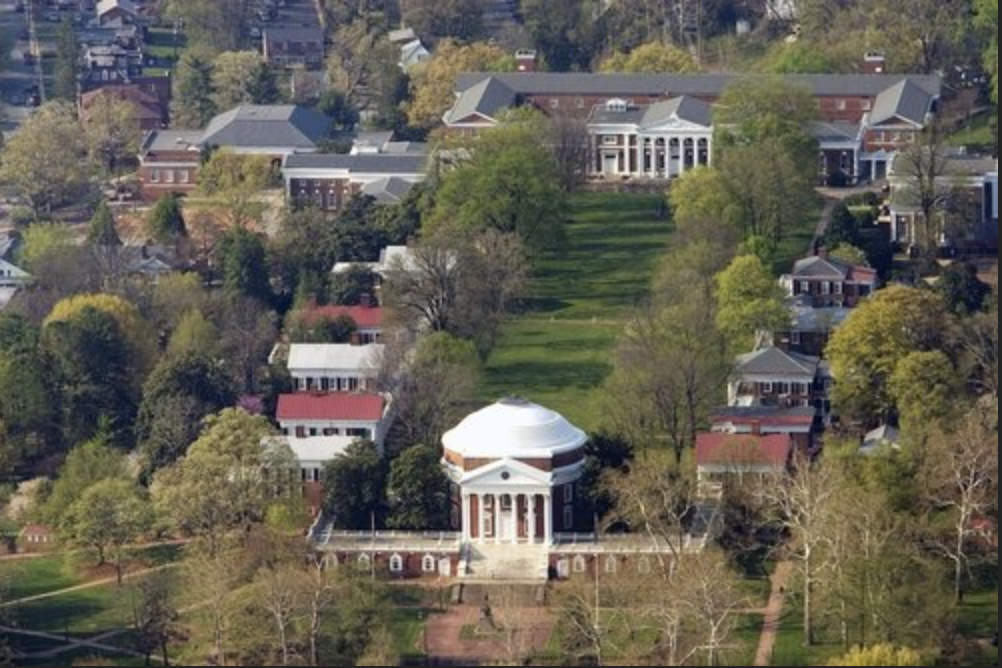
\includegraphics[width=4.16667in,height=\textheight]{images/UVA.png}

UVA Library:

\begin{itemize}
\tightlist
\item
  Our team members come from Scholarly Communications and Research Data
  Services \& Social, Natural, and Engineering Sciences, which are teams
  from different units in the library.
\item
  Research Data Services has a long-running workshop series.
\item
  It is very rare for library staff to teach for-credit courses at UVA.
\end{itemize}

\note{JENN: 1 min (spend 1 minute here)

Welcome to our talk today about how we implemented a Reproducibility
workshop series at UVA Library. I am Jennifer Huck; I'm the Data
Librarian and Acting Associate Director of Research Data Services at UVA
Library. I am joined by Sherry Lake, the Scholarly Repository Librarian,
and Erich Purpur, a Science and Engineering Research Librarian.

Here is a little about the University of Virginia:

\begin{itemize}
\tightlist
\item
  R1 university.
\item
  There are about 23,000 students and there are 12 Schools.
\item
  Only the School of Data Science has a policy for open access and open
  data
\end{itemize}

And some context for UVA Library:

\begin{itemize}
\tightlist
\item
  Our team members come from Scholarly Communications and Research Data
  Services \& Social, Natural, and Engineering Sciences, which are teams
  from different units in the library.
\item
  Research Data Services has a long-running workshop series on tools for
  quantitative and qualitative data analysis.
\item
  One thing to point out: It is very rare for library staff to teach
  for-credit courses at UVA. Teaching a within a workshop series like
  this is one of our best chances for instruction.
\end{itemize}}
\end{frame}

\begin{frame}{What We Did}
\protect\hypertarget{what-we-did}{}
A \textbf{new workshop series}: `Reproducible Research for Early
Graduate Students'

Included 2 \textbf{technical} and 2 \textbf{non-technical} sessions:

\begin{itemize}
\tightlist
\item
  Technical sessions: tools and workflows
\item
  Non-Technical sessions: conceptual instruction on organization and
  data sharing
\end{itemize}

\note{JENN: 3 min (spend 2 minutes here)

\begin{itemize}
\tightlist
\item
  In Spring 2021, UVA Library's Research Data Services (RDS) launched a
  \textbf{new workshop series} called ``Reproducible Research for Early
  Graduate Students.''
\item
  The overall concept was to enable researchers to improve data use and
  re-use for collaborators and themselves; to use available technical
  tools to create reproducible workflows; and to communicate and
  disseminate findings and data. The initial target audience was early
  graduate students in STEM departments.
\item
  The four workshops in the series focused on both \textbf{technical}
  and \textbf{non-technical tools for reproducible research}.

  \begin{itemize}
  \tightlist
  \item
    Our technical sessions covered tools and workflows, and
  \item
    Our non-technical sessions covered file and metadata organization
    and data sharing.
  \end{itemize}
\end{itemize}}
\end{frame}

\begin{frame}{How We Did It}
\protect\hypertarget{how-we-did-it}{}
\begin{itemize}
\tightlist
\item
  We launched it as a \textbf{standalone mini-series} as part of
  Research Data Service's ongoing workshop series
\item
  We leveraged a relatively \textbf{varied skillset} among library staff
  to present these sessions.
\item
  Sessions were a mix of \textbf{old} and \textbf{new} workshop content
\item
  Outreach: Research Data Services Newsletter, reaching out to
  communications directors at various schools
\item
  Virtual (Spring 2021) and In Person (Fall 2021)
\end{itemize}

\note{JENN: 4 min (spend 1 min here)

\begin{itemize}
\tightlist
\item
  Each semester, our Research Data Services team presents an extensive
  suite of workshops taught by our staff, as well as collaborators from
  other units throughout the university. We offer training on technical
  tools, such as R, Python, Tableau, and Dedoose. We launched our
  Reproducibility series as a \textbf{standalone mini-series} within
  that workshop environment.
\item
  We are fortunate to have a lot of staff at our library with some
  facility in data. We were able to pull in librarians with
  \textbf{varied skillsets}.
\item
  Our sessions were a mix of old and new workshop content. Of the
  sessions in our reproducibility series, one was an existing workshop,
  one was a mashup of old and new content, and two were brand new.
\item
  As for Outreach, we advertised the sessions in our Research Data
  Services Newsletter which goes out to interested readers at UVA, and
  we also reached out directly to communications directors at various
  schools who then send info to their students.
\item
  We had two presentation formats. This Spring, we presented virtually
  via Zoom, and this Fall we presented in person.
\end{itemize}}
\end{frame}

\hypertarget{workshop-details-non-technical-sessions}{%
\section{Workshop Details: Non-Technical
Sessions}\label{workshop-details-non-technical-sessions}}

\begin{frame}{Organizing Files and Metadata for Transparent \&
Reproducible Research}
\protect\hypertarget{organizing-files-and-metadata-for-transparent-reproducible-research}{}
\begin{itemize}
\tightlist
\item
  Project organization: demonstrated \& discussed the concepts

  \begin{itemize}
  \tightlist
  \item
    Organizing files: directory (grouping) structure
  \item
    Documentation (e.g., READMEs)
  \item
    File Naming
  \end{itemize}
\end{itemize}

\note{SHERRY: 5 min (spend 1 min here)

The workshop series started with the non-technical workshop: Organizing
Files and Metadata for Transparent \& Reproducible Research

In this workshop, participants were instructed on fundamental approaches
on creating a research compendium, which is the foundation of
transparent and reproducible research.

Participants learned what kinds of documents and materials they should
create and preserve; what type of information the documents should
contain; and how they should be formatted and organized. Topics for this
workshop included organizing raw data (files), data analysis,
documentation, scripts, metadata, readme files, project organization,
and naming conventions.

The examples were based in R, but no programming experience or
experience with R was required, as the information learned in the
workshop could be applied to any quantitative programming environment.}
\end{frame}

\begin{frame}{Sharing Your Data for Transparent and Reproducible
Research}
\protect\hypertarget{sharing-your-data-for-transparent-and-reproducible-research}{}
\begin{itemize}
\tightlist
\item
  Why share
\item
  Where to share

  \begin{itemize}
  \tightlist
  \item
    Picking a repo
  \item
    Introducing FAIR principles
  \end{itemize}
\item
  What to share
\item
  How to Share
\item
  List of steps for sharing
\end{itemize}

\note{SHERRY: 6 min (spend 1 min here)

The last workshop in the series was Sharing Your Data for Transparent
and Reproducible Research

This workshop covered tools and resources on sharing research during a
project and at the completion of a project. Participants learned why,
how and where to share and disseminate research results per funder and
journal requirements. Topics covered included introducing the Open
Science Framework (OSF), making your research data FAIR, locating
repositories to disseminate research, and licensing data.

This workshop was broken down into why, where, what, how, when to share
data.

Starting with an overview of why share, which included among other
reasons, the need to share for transparency.

It included - Where to share How to pick a repository By Introducing
FAIR principles - as way to select a repo \& talk about ``re-use'' \&
how it relates to transparency.

What to share - covered what can't be shared \& included a list of UVa's
policies related to data collection and data protection.

How to Share, including licenses - keying in on the purpose of sharing
for Transparent and reproducible research (for our workshops at least)

This is where I related ``Sharing'' to a Data Management or Sharing
Plan. Sharing Starts w/ these - key Data Management practices, those
practices from the earlier workshop on organization and version control.

The Sharing session concluded w/ a summation list of steps for sharing.}
\end{frame}

\hypertarget{workshop-details-technical-sessions}{%
\section{Workshop Details: Technical
Sessions}\label{workshop-details-technical-sessions}}

\begin{frame}{Version Control with Git and GitHub}
\protect\hypertarget{version-control-with-git-and-github}{}
\begin{itemize}
\tightlist
\item
  Learn about version control
\item
  Install git and make Github account
\item
  Common workflow scenarios

  \begin{itemize}
  \tightlist
  \item
    local changes
  \item
    push to remote repository
  \item
    branching/collaboration
  \end{itemize}
\end{itemize}

\note{ERICH: 7 min (spend 1 min here)

I taught the workshop on version control using Git and Github. Version
control is used to manage code development individually or in a team
setting. In the context of this presentation, version control is really
important because it is basically a complete record of everything that
has happened in your code base since the beginning of a project. We
first made sure that everyone was up and running with Git and also a
github account. Then we walked through common workflow scenarios. We
first tracked our code changes locally. Then we pushed the to the remote
Github repository. Later, we walked through collaboration scenarios
using branches and pull requests.}
\end{frame}

\begin{frame}{RStudio and R Markdown}
\protect\hypertarget{rstudio-and-r-markdown}{}
\begin{itemize}
\tightlist
\item
  Review RStudio Projects to create a project-oriented workflow in R.
\item
  Overview of R Markdown for literate programming, including new
  features of Visual R Markdown.
\end{itemize}

\note{JENN: 8 min (spend 1 min here)

For this session we reviewed RStudio Projects to create a
project-oriented workflow in R. We also provided an overview of R
Markdown for literate programming. This highlighted the new features of
Visual R Markdown, which makes using R Markdown much easier and has some
great new features like connecting RStudio to Zotero.}
\end{frame}

\begin{frame}{How You Can Do It}
\protect\hypertarget{how-you-can-do-it}{}
\begin{itemize}
\tightlist
\item
  Look for partners at your institution to partner with
\item
  You don't need to be an expert - skills can be emerging
\item
  Re-brand existing workshops and classes at your library
\item
  Take our stuff!
\end{itemize}

\note{JENN: 10 min (spend 2 min here)

Here are some takeaways:

\begin{itemize}
\tightlist
\item
  Look for partners to collaborate on a series of reproducibility. One
  person does not and should not have to do it all! We partner with
  other library colleagues outside of Research Data Services and units
  outside of the library. For example, we collaborate with librarians
  like Sherry, who is not a part of Research Data Services and also with
  our Health Sciences Library and Research Computing colleagues to offer
  a wide variety of workshops.
\item
  We all have various levels of technical expertise. Some technical
  experience is definitely helpful but you don't have to be a data
  scientist to teach in this area. I consider my skills in R to be
  ``emerging,'' but I found that that was enough for me to ``see'' the
  value in tools (especially in RStudio) or concepts that might be
  overlooked or not formally taught. Not all these tools require a
  strong statistical, data science, or programming background in order
  to teach them.
\item
  Look around for existing workshops at your library to market or
  re-brand to fit into a Reproducibility theme. Are you already doing
  things you could use for this purpose? Sherry will expand on this idea
  in the next slide.
\item
  Finally, all of our workshop material is openly available. Take our
  stuff! There is no need to create all the materials from scratch. Note
  that the version control workshop is a combination of previous
  workshop materials plus online content that created externally.
\end{itemize}}
\end{frame}

\begin{frame}{Transform Data Management Workshops}
\protect\hypertarget{transform-data-management-workshops}{}
\begin{figure}
\centering
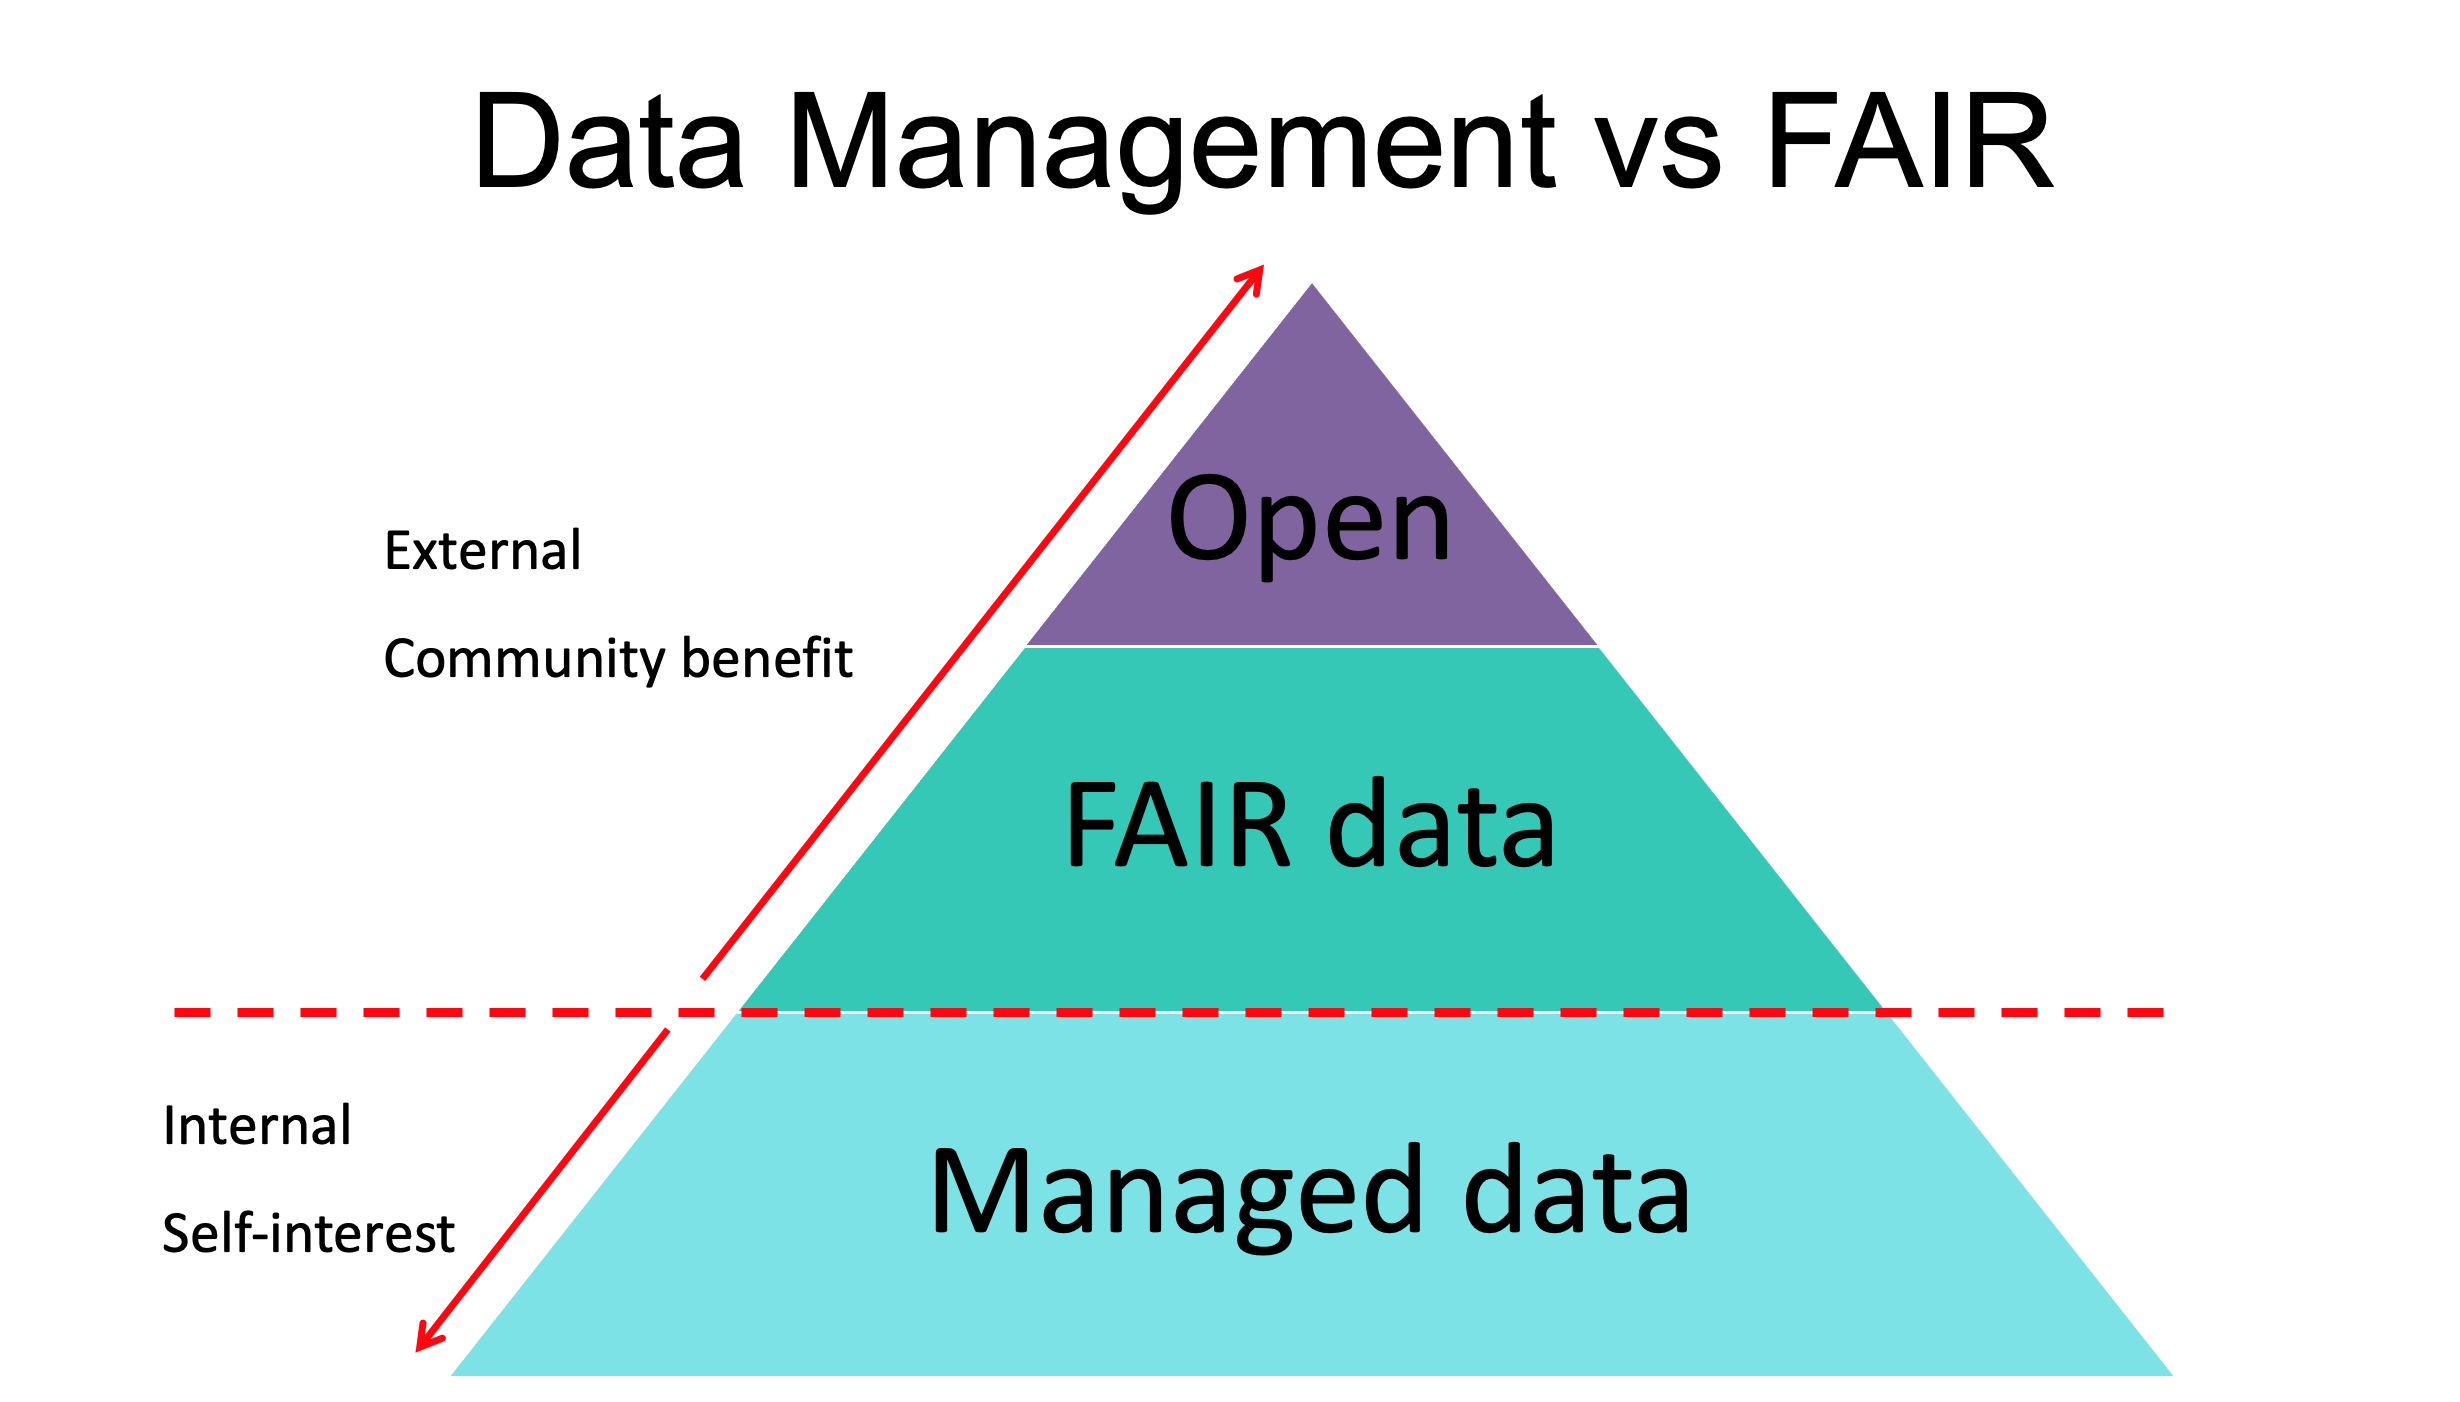
\includegraphics[width=7.8125in,height=\textheight]{images/DM_vs_FAIRSharing.png}
\caption{(\protect\hyperlink{ref-jones_open_2018}{Jones 2018})}
\end{figure}

\note{SHERRY: 12 min (spend 2 min here)

I want to spend a couple of minutes making a link from typical data
management and sharing workshops to transparency and reproducibility.

Doing research for transparency and managing data (data management)
{[}and FAIR{]} are overlapping, but distinct concepts each emphasizing
different aspects of handling and sharing research data.

Knowing about these ``differences'' (and strengths) can help librarians
promote good research practices. Sharing - promote access \& reuse, DM
is basis from the start of a project in order for sharing to be
meaningful.

Research Data Management (RDM): is not a goal in itself, but a set of
practices to handle information collected and created during research.
RDM is the compilation of many small practices that make your data
easier to find, easier to understand, less likely to be lost, and more
likely to be usable during a project or ten years later.

FAIR principles advocate for increased findability, accessibility,
interoperability and reusability of research data and scholarly digital
objects more generally.

FAIR and transparency are ``noble'' aspirations \& useful way to engage
researchers and encourage good data practices from the outset.
FAIR/Reproducibility are more catchy concepts to engage researchers in
DM.

FAIR and transparency extends DM - data \& research is not just managed
but are FAIR and can be understood, reproducible. Data that is not
``managed'' cannot be successfully shared/re-used (FAIR).

Thus\ldots{} we can't forget data management - DM is needed before data
can be FAIR and shared - it enables data to be created and used in a way
that increases transparency helps in sharing and reuse. BUT\ldots. maybe
by using the more appealing language of FAIR and organizing research, we
can engage researchers in data management too. Note: Jenn did not use
the phrase ``Data Management'' at all in her workshop/title or
presentation, BUT file organization, file naming, documentation are all
basic DM 101.

FAIR and transparency both focus on data sharing, ensuring content is
made available in ways that promote access and reuse. Data management by
contrast is about the stewardship of data from the point of conception
onwards. It makes no assumptions about access, but is essential if data
are to be meaningful to others.

The way we presented the concepts of reproducible research \& sneaking
in DM concepts (without calling them that) and FAIR practices is a
useful way to engage researchers and encourage good data practices from
the outset. It might open conversations with researchers and funders in
ways that dull old data management never did.

Research Data Management is the foundation for sharing. Managing and
sharing research data are not a high priority for researchers - choosing
the right ``terminology'' (concepts of FAIR, organization, sharing,
transparency, reproducibility) can help in the up-take of best practices
for managing and sharing.}
\end{frame}

\begin{frame}{Resources To Start With}
\protect\hypertarget{resources-to-start-with}{}
\begin{itemize}
\tightlist
\item
  Practical Reproducibility

  \begin{itemize}
  \tightlist
  \item
    Transparent and Reproducible Social Science Research
    (\protect\hyperlink{ref-christensen2019}{Christensen 2019})
  \item
    Inspiration for a multi-part course on Reproducibility: Reproducible
    Research Techniques for Synthesis:
    (\protect\hyperlink{ref-nationalcenterforecologicalanalysisandsynthesis}{National
    Center for Ecological Analysis and Synthesis, n.d.})
  \end{itemize}
\item
  Organize for Transparent and Reproducible Research

  \begin{itemize}
  \tightlist
  \item
    Reproducible Science Curriculum: Data \& Project Organization
    (\protect\hyperlink{ref-datacarpentry}{Data Carpentry, n.d.})
  \item
    How to Name Files (\protect\hyperlink{ref-bryan2015}{Bryan 2015})
  \end{itemize}
\item
  Version Control with Git and GitHub

  \begin{itemize}
  \tightlist
  \item
    Git Command Line Basics
    {[}\url{https://www.youtube.com/watch?v=HVsySz-h9r4}{]}
  \end{itemize}
\item
  Sharing Your Data for Transparent and Reproducible Research

  \begin{itemize}
  \tightlist
  \item
    Data Management vs FAIR (\protect\hyperlink{ref-higman2019}{Higman,
    Bangert, and Jones 2019})
  \item
    Best Practices
    (\protect\hyperlink{ref-briney_foundational_2020}{Briney, Coates,
    and Goben 2020})
  \end{itemize}
\item
  Reproducible Analysis and Documentation in RStudio and R Markdown

  \begin{itemize}
  \tightlist
  \item
    Reproducible Research With R and RStudio
    (\protect\hyperlink{ref-gandrud2020}{Gandrud 2020})
  \end{itemize}
\end{itemize}

\note{ERICH: 13 min (spend 1 min here)

Here are a few high-level resources that we like. Our workshop slides
contain more detailed references.}
\end{frame}

\begin{frame}{Feedback and Assessment}
\protect\hypertarget{feedback-and-assessment}{}
\begin{itemize}
\tightlist
\item
  Track attendance
\item
  Post workshop follow up
\end{itemize}

\note{ERICH: 14 min (spend 1 min here)

Graduate students are our target audience and most common attendee type
but we had a lot of attendees who were post-docs and research
scientists, which we did not expect.

We also have a number of post-docs, faculty, staff, undergraduates, and
community members.

In the pre-covid times we held in-person workshops and attendance has
traditionally been high. During the pandemic last year, we taught our
workshops online with good attendance. This semester, the university is
pushing hard to go ``back to normal'' so we have been offering our
workshops in person again. Attendance has been low and we feel it is
probably just too soon for the full in-person workshops again.}
\end{frame}

\begin{frame}{Looking Forward}
\protect\hypertarget{looking-forward}{}
Some ideas:

\begin{itemize}
\tightlist
\item
  Do specific outreach to departments on this kind of training
\item
  Find a seminar series that this could fit into
\item
  Find ``reproducibility champions'' who want their grad student to
  learn these concepts
\end{itemize}

\note{JENN: 15 min (spend 1 min here)

\begin{itemize}
\tightlist
\item
  We would consider trying to take this to specific departments, by
  reaching out to Directors of Graduate Studies.
\item
  We might also find other seminar series at UVA where this might fit
  into.
\item
  A final idea is to find Reproducibility champions who want their grad
  students to learn these concepts, and come teach a lab directly.
\end{itemize}}
\end{frame}

\begin{frame}{More Resources}
\protect\hypertarget{more-resources}{}
\begin{itemize}
\tightlist
\item
  Our Workshop materials are available at OSF:
  \url{https://osf.io/ws3u2}

  \begin{itemize}
  \tightlist
  \item
    There are considerably more references to learn more about each
    individual topic in the workshop slides
  \end{itemize}
\item
  Research Data Management Services Zotero group library:

  \url{https://www.zotero.org/groups/361046/research_data_management_services/library}
\end{itemize}

\note{JENN: x min (spend 0 min here)

\begin{itemize}
\tightlist
\item
  All our workshop material can be found at OSF.
\item
  If you are interested in learning more about Research Data Management
  Services, we recommend this great Zotero library.
\end{itemize}

That's it! Thanks for coming to our talk.}
\end{frame}

\begin{frame}{References}
\protect\hypertarget{references}{}
\hypertarget{refs}{}
\begin{CSLReferences}{1}{0}
\leavevmode\hypertarget{ref-briney_foundational_2020}{}%
Briney, Kristin, Heather Coates, and Abigail Goben. 2020.
{``Foundational {Practices} of {Research Data Management}.''}
\emph{Research Ideas and Outcomes} 6 (July): e56508.
\url{https://doi.org/10.3897/rio.6.e56508}.

\leavevmode\hypertarget{ref-bryan2015}{}%
Bryan, Jenny. 2015. {``How to Name Files.''} \emph{Speaker Deck}.
https://speakerdeck.com/jennybc/how-to-name-files.

\leavevmode\hypertarget{ref-christensen2019}{}%
Christensen. 2019. \emph{Transparent and {Reproducible Social Science
Research}}. First edition. {Oakland, California}: {University of
California Press}.

\leavevmode\hypertarget{ref-datacarpentry}{}%
Data Carpentry. n.d. {``Reproducible {Science Curriculum}: Data \&
{Project Organization}.''}
https://reproducible-science-curriculum.github.io/organization-RR-Jupyter/.

\leavevmode\hypertarget{ref-gandrud2020}{}%
Gandrud, Christopher. 2020. \emph{Reproducible {Research} with {R} and
{RStudio}}. 3rd edition. {Boca Raton, FL}: {Chapman and Hall/CRC}.

\leavevmode\hypertarget{ref-higman2019}{}%
Higman, Rosie, Daniel Bangert, and Sarah Jones. 2019. {``Three Camps,
One Destination: The Intersections of Research Data Management, {FAIR}
and {Open}.''} \emph{Insights} 32 (1): 18.
\url{https://doi.org/10.1629/uksg.468}.

\leavevmode\hypertarget{ref-jones_open_2018}{}%
Jones, Sarah. 2018. {``Open Data, {FAIR} Data and {RDM}: The Ugly
Duckling.''} {Berlin}. \url{https://doi.org/10.5281/zenodo.1196631}.

\leavevmode\hypertarget{ref-nationalcenterforecologicalanalysisandsynthesis}{}%
National Center for Ecological Analysis and Synthesis. n.d.
{``Reproducible {Research Techniques} for {Synthesis}.''} \emph{National
Center for Ecological Analysis and Synthesis}.
https://www.nceas.ucsb.edu/learning-hub/short-course.

\end{CSLReferences}
\end{frame}

\end{document}
